If a group of informed individuals are moving in the \emph{front line} of the group, these informed group will walk in a circular shape, making a quadratic bounding box surrounding them. 
The rest of the group will follow the informed group, so that if there are the same number of uninformed individuals as informed, they will together make up a bounding box with elongation of about 2, meaning that the side of the bounding box parallel to the direction is twice as long as the side perpendicular to the direction.
\newcommand{\figwidth}{0.21\textwidth}
\begin{figure}[H]
	\centering
	\begin{subfigure}[b]{\figwidth}
		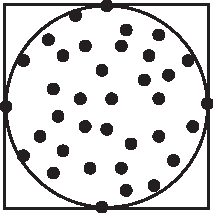
\includegraphics[width=\textwidth]{img/Circle.pdf}
		\caption{Actual distribution in box.\\\ }
		\label{fig:hitratio-nb}
	\end{subfigure}
	~
	\begin{subfigure}[b]{\figwidth}
		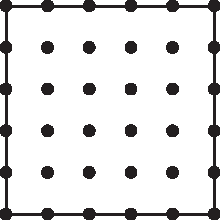
\includegraphics[width=\textwidth]{img/Square.pdf}
		\caption{Analytically approximated distribution}
		\label{fig:hitratio-mn}
	\end{subfigure}
	\caption{Hit ratio as a function of vocabulary size after $\chi^2$ feature selection for different classifiers and data types.}
	\label{fig:hitratio}
\end{figure}

\begin{figure}[H]
	\centering
	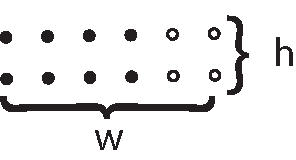
\includegraphics[width=0.24\textwidth]{img/heightwidth.pdf}
	\caption{Here is stuff.}
	\label{fig:hitratio}
\end{figure}